\section{Considerações finais}
\begin{frame}{Considerações finais}
	\begin{columns}[t]
		\column{5cm}
			\begin{figure}[tb]
				\centering
				\caption{Ambiente do Google Colaboratory com o conteúdo de neurônios de disparo}
				\label{fig:colab}
				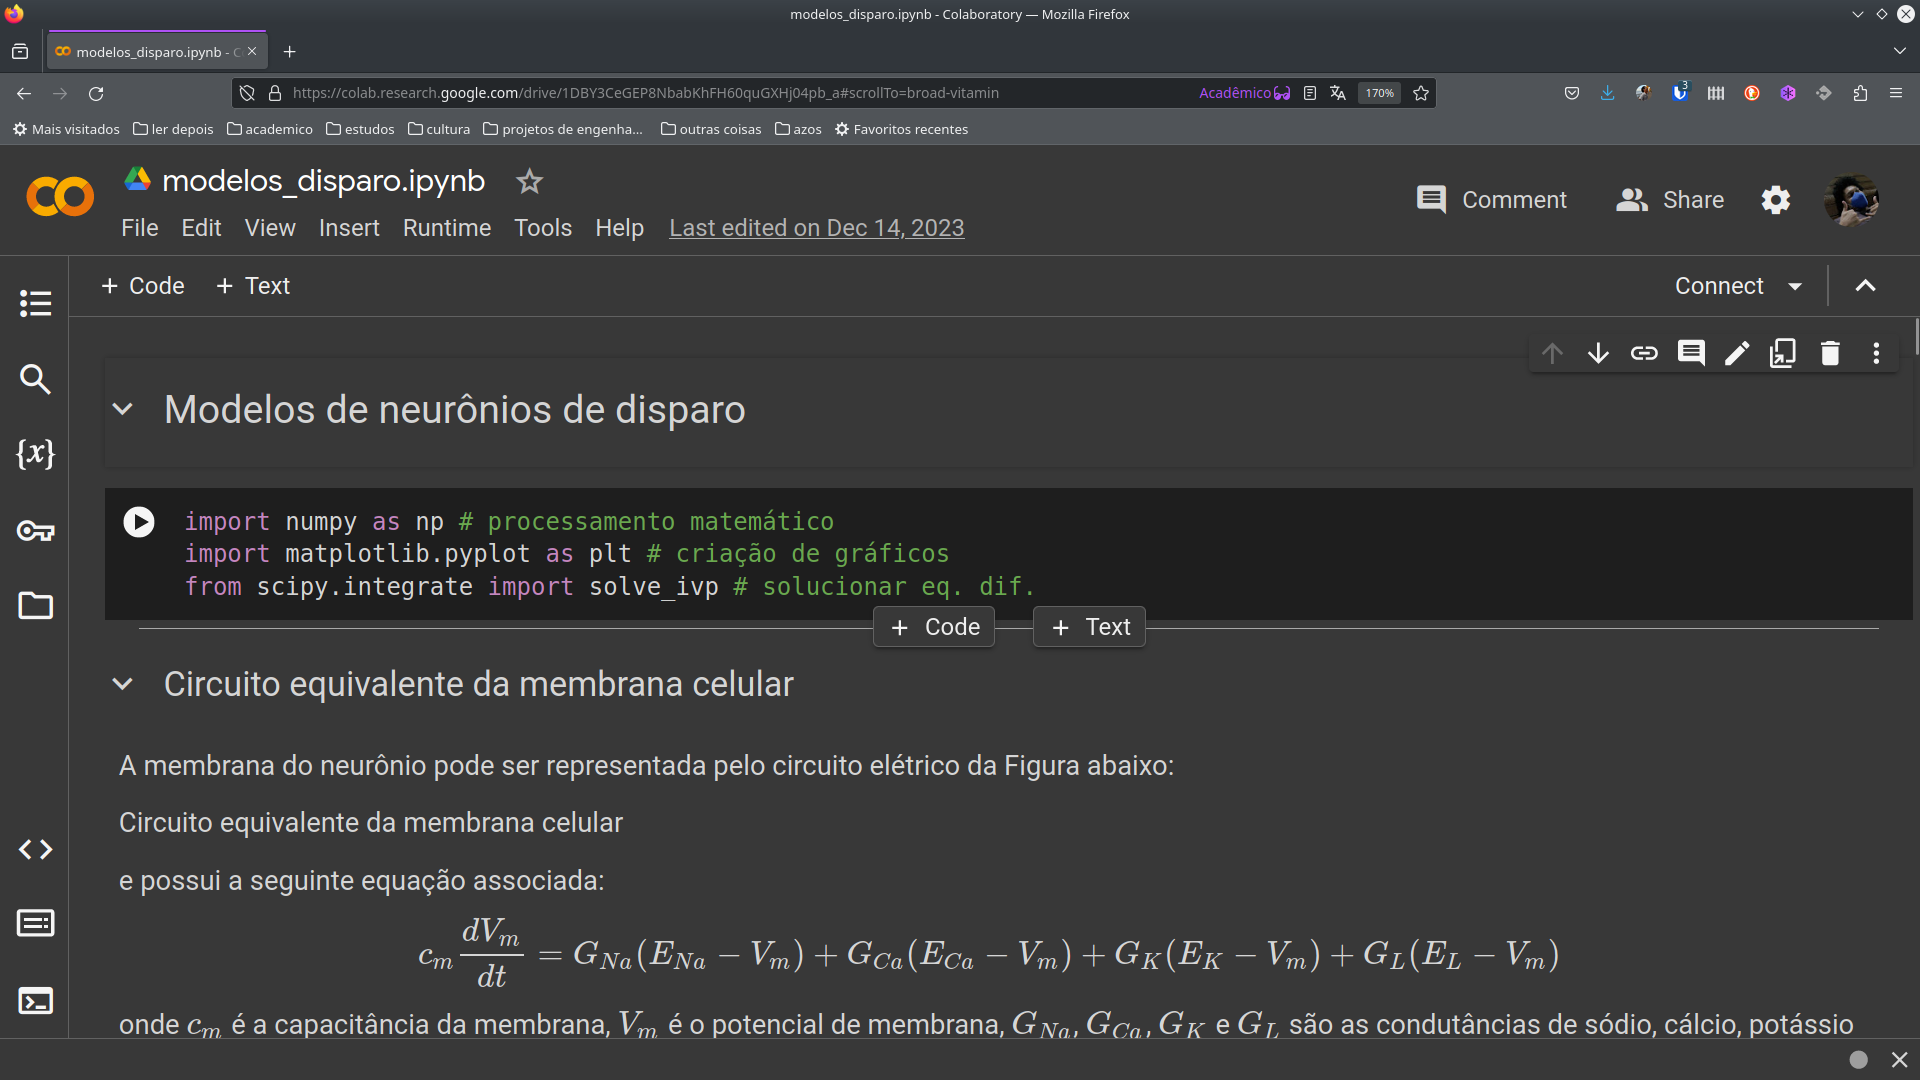
\includegraphics[width=\linewidth]{figs/colab}
%				\legend{Fonte: o autor (\the\year)}
			\end{figure}
		\column{5cm}
			\begin{itemize}
				\item Proposta de sequência didática gerada;
				\note{sequencia didatica: incluindo atividades avaliativas}
				\item códigos fontes em repositório online;
				\note{codigos fonte: incluindo os que geram algumas figuras do texto}
				\item novos conteúdos podem incluir a estimulação elétrica axonal, a análise de sinais de eletroencefalograma (EEG) e a apresentação de pacotes voltados à simulação neuronal.
				\note{estimulação elétrica: estudar a propagação do potencial de ação ao longo do axônio}
				\note{eeg: respostas elétricas obtidas das atividades cerebrais. podem ser utilizadas para associações com comorbidades, como depressão e ansiedade}
				\note{pacotes: tem seu entendimento facilitado pós conteúdo deste curso}
			\end{itemize}
	\end{columns}
\end{frame}
